\documentclass[pdftex,10pt,a4paper,oneside]{article}
%Can change the pt, papersize etc.
\usepackage{listings}
\usepackage{amsmath}
\usepackage{amssymb}
\usepackage{algorithm}
\usepackage{algorithmic} %Algorithm styles, need to be nested for the example shown
\usepackage{fancyhdr} %For our headers
\usepackage{graphicx} %Inserting images
\usepackage{lipsum}  %Blank text fill, delete me when finished
\usepackage{setspace} %Spacing on the front page for crest and titles
\usepackage[]{fncychap} % Styles can be Sonny, Lenny, Glenn, Conny, Rejne, Bjarne and Bjornstrup
\usepackage[hyphens]{url} %Deals with hyphens in urls to make them clickable
\usepackage{xcolor} %Great if you want coloured text
\usepackage{tabularx}
\usepackage{appendix} %Take a wild guess slick

%KEEP THIS ONE LAST it's quite buggy, it allows you to click on links within the pdf and web links without changing the colour. The mouse cursor simply changes its icon to indicate to the user. Great tool - still awkward
\usepackage[hidelinks]{hyperref}


%This will tell the compiler to do the header style, page and spacing between the header and text
\fancyhf{}
\renewcommand{\headrulewidth}{0.2pt}




% Load the package
\usepackage[toc]{glossaries}

% Generate the glossary
\makeglossaries
%\includeonly{%chapters/ch1.tex,
%	chapters/ch3.tex,
%	chapters/ch4.tex,
%	chapters/ch5.tex,
%	chapters/ch6.tex,
	%chapters/ch7.tex,
	%chapters/ch8.tex,
	%chapters/ch9.tex,
	%chapters/ch10.tex,
%	chapters/ch11.tex,
%	chapters/ch12.tex,
	%chapters/ch13.tex,	}
\begin{document}
	
	\pagenumbering{arabic}
	
	\begin{spacing}{2}
		\begin{center}
			
\includegraphics[scale = 0.20]{ASU.png}
		\end{center}
		\vspace{5mm}
		\begin{center}
			\textbf{\begin{LARGE}
					Conan:Finding missing people
			\end{LARGE}}
			\vspace{2mm}
		\end{center}
		\begin{center}
			\textbf{\large Mohamed Atta Ibrahim \\Mohamed Yasser Ahmed 
				\\Mahmoud Mohamed Benyamin \\ Hady Ashraf Ragab\\Yousef Abdelbadea Ali}
			\vspace{2mm}
		\end{center}
		\begin{center}
			\textbf{\large Supervisor:Dr. Mahmoud Khalil
			 }\\
			\textbf{\large Department of Computer and Systems Engineering}\\
			\textbf{\large Faculty of Engineering at Ain Shams University}\\
			
			{\large \today\\}
		\end{center}
	\end{spacing}
	
	\pagebreak
	
	\tableofcontents
	\pagebreak
	\listoffigures
	\pagebreak
	\listoftables
	\pagebreak
	\begin{abstract}{
			This paper presents imp DIP project
	}	\end{abstract}
	\pagebreak
	\section*{Introduction}
In this project the user can find missing people by search with the old pictures or young pictures of missing people. The project uses techniques that extract features from the pictures and check similarity between the query picture and the pictures in the dataset to retrieve the similar picture to the query picture.
	 
	\addcontentsline{toc}{section}{Introduction}
	
	
	\pagebreak
	
	\section{project description}
	This is a python desktop application, it applies the Pattern Recognition and	Digital Image Processing
	 techniques to analyze, design, and implement multimedia retrieval system, where the media that we are going to use are the images .we have implemented many techniques belong  Pattern Recognition and Digital Image Processing and AI techniques in retrieval and face Recognition.
	 .
	\begin{figure}[H]
		\centering
		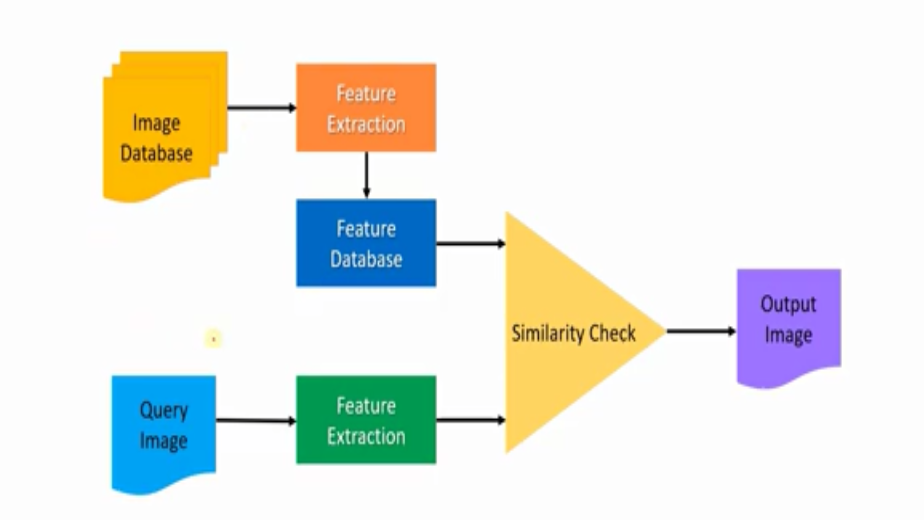
\includegraphics[width=120mm,height=60mm]{fig/19.png}
		\caption{image system block diagram }
		\label{image system block diagram}
	\end{figure}

	\pagebreak
	\section{Beneficiaries of the project}
	The family who want to find any one of their members because of missing of him.
	Any one who the government wants to find from his traffic camera's pictures to detect his data and find him.

	
	\pagebreak
	\section{Detailed analysis}
	This project deals with Content Based Image Retrieval(CBIR). For the CBIR, the adopted method is face recognition and then after the user provide the image(person) that he/she want to search for. The program extract features of the images dataset and save it then extract the features of the input image and compare the image with extracted feature database(persons saved in dataset) and after that compares it using Intersection Distance method to detect the closet person for input images and his/her information (if it was inserted to the database)
	
	\subsection{Face recognition}
	Face recognition software use computer algorithms to determine specific, distinguishing features on a human's face Some features, like eyeball proximity or jaw shape, would then be transformed into a mathematical model and analyzed to data from other faces in a face recognition dataset. A face template is data on a specific face that differs from an image in that it is designed to only include certain traits that could be used to recognize a face over others 
\begin{figure}[H]
	\centering
	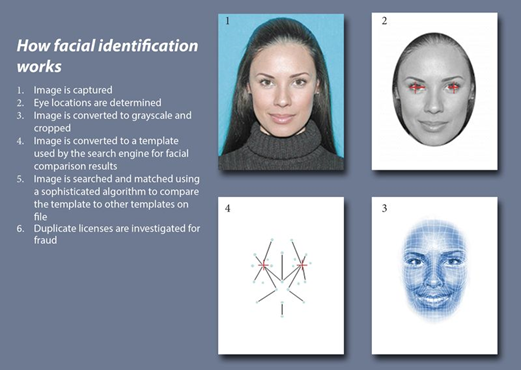
\includegraphics[width=120mm,height=60mm]{fig/30.png}
	\caption{Face recognition  }
	\label{Face recognition }
\end{figure}
Rather than precisely recognizing an unidentified individual, certain facial recognition technologies are intended to compute a probabilistic match score between both the unidentified individual and certain face templates stored in the dataset. Rather than providing a single result, such algorithms will present numerous probable matches, sorted in order of probability of right identification.\\
Facial recognition systems differ in their capacity to recognize persons under difficult situations, including such dim lighting, poor picture quality, as well as a skewed angle of view (such as in a photograph taken from above looking down on an unknown person).\\
When it comes to errors, there are two key concepts to understand: \\
Whenever a facial recognition system fails to capture an individual's face to a picture which is in fact stored in the dataset this is known as a "false negative." In other terms, the algorithm will respond to a query with zero results, which is incorrect.\\
Whenever a facial recognition algorithm matches a human's face to a picture inside a dataset, however the similarity is inaccurate, it's called a "false positive." If a policeman sends an image of "Joe," the system incorrectly informs the cop that the image is of "Jack."\\
While looking into a facial recognition algorithm pay special attention towards the "false positive" and "false negative" ratios, because there is almost always an exchange. When you use facial recognition to unlock your device, for example, it's preferable if the algorithm misidentifies you a few occasions (false negative) than for the system to misidentify other individuals as you and allow them to access your mobile (false positive). If a mistaken identity leads to the incarceration of an innocent individual (such as a mugshot database misidentification), the system must be developed to get as few false positives as possible.

some distance that we used to measure similarity 
\begin{itemize}
	\item Absolute Distance \\
	\begin{equation}
		D_{Absolute}(h,\bar{h})= \sum_{K-1}^{K} |h_{K}-\bar{h_{K}}|
	\end{equation}
	\item Euclidean Distance \\
	\begin{equation}
		D_{Euclidean}(h,\bar{h})= \sqrt{\sum_{K-1}^{K} (h_{K}-\bar{h_{K}})^{2}}
	\end{equation}
	\item Intersection Distance \\
	\begin{equation}
	D_{Intersection}(h,\bar{h})= 1- \sum_{K-1}^{K} in(h_{K},\bar{h_{K}})
	\end{equation}
	
	
	
\end{itemize}


	
	\pagebreak
	\section{Detailed description of the adopted techniques }
	For face recognition we use face recognition library part of dlib
	we detect features of persons faces ex (eye color , eye size , iris , face parts ratios ) using face recognition from dlib to extract features and then save them in .csv file
	
	
	
	
		\textbf{{\large steps}}\\
		\begin{enumerate}
			\item Resize image to make it take less time
			
			
		
			
			
			
			\item Turn it to gray 
			\item Extract features
			\item Save features in .csv file
			\item (optional) add information for the person in the image to add it to our database so it’ll appear when we search through  images
			
		\end{enumerate}







	
	\textbf{{\large distance}}\\
	we use Intersection Distance error method to compare between the image we search for (after extracting features)  and features of the images saved in database\\
	Intersection Distance \\
	\begin{equation}
		D_{Intersection}(h,\bar{h})= 1- \sum_{K-1}^{K} in(h_{K},\bar{h_{K}})
	\end{equation}
	
	Meaning the lower the distance the better (closer to image we search for)
	\pagebreak

		
	\pagebreak
	\section{Time plan}
In Prepairing Datasets phase, We search for qualified dataset that qualify project.
In parrallel, Extraction Features Algorithms design are finished. The software is
developed and then make testing for all functionality of the
program.

	
	\begin{figure}[H]
		\centering
		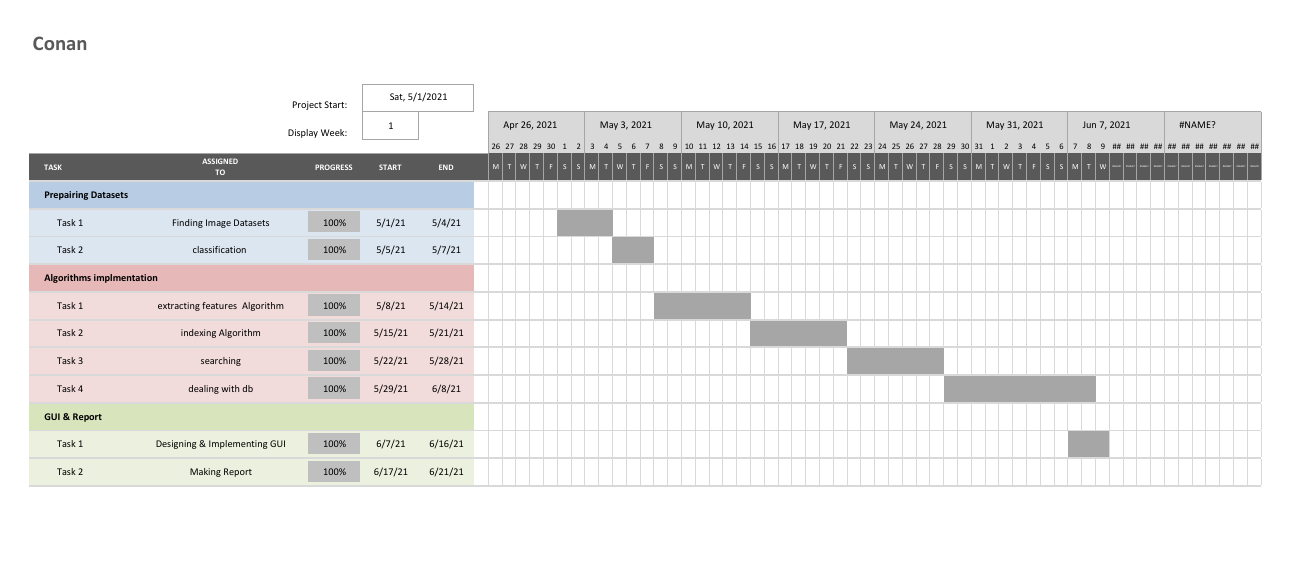
\includegraphics[width=140mm,height=80mm]{fig/5.png}
		\caption{time plan }
		\label{time plan}
	\end{figure}
	\pagebreak
	\section{System architecture}
		\begin{figure}[H]
		\centering
		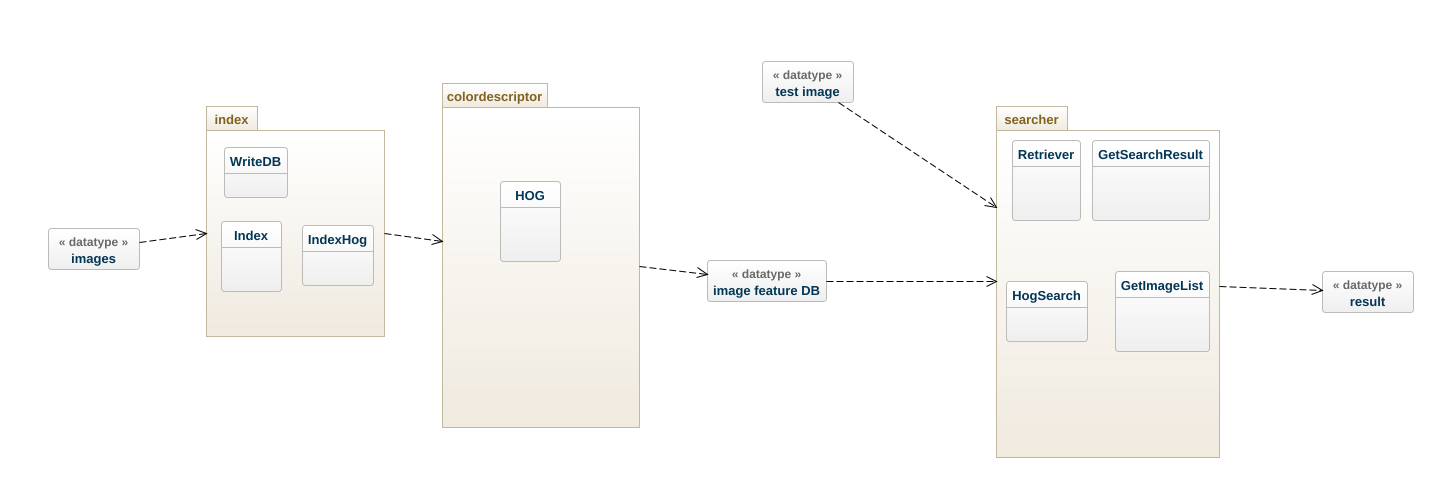
\includegraphics[width=140mm,height=80mm]{fig/22.png}
		\caption{System architecture class-diagram }
		\label{System architecture class-diagram}
	\end{figure}

\begin{figure}[H]
	\centering
	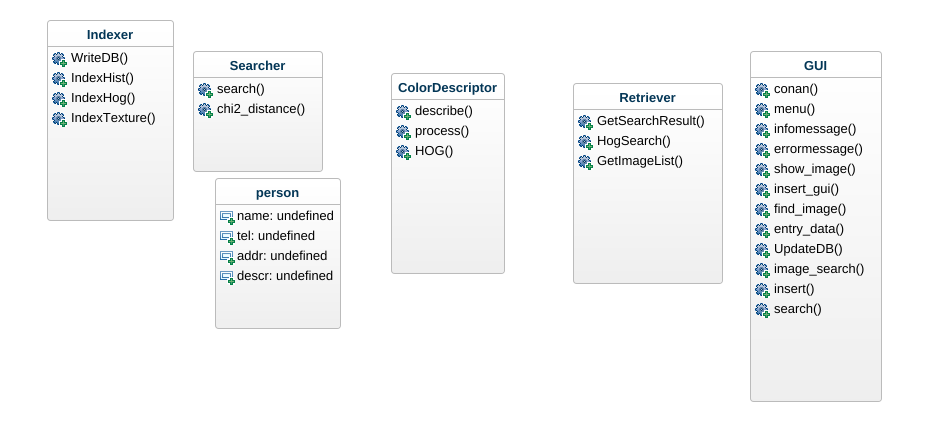
\includegraphics[width=140mm,height=80mm]{fig/23.png}
	\caption{class-diagram }
	\label{class-diagram}
\end{figure}

\pagebreak
	\section{database design}
	\begin{itemize}
		\item We implemented the schema in sqlite and store features in csv file which ID is the path of the image.
			\begin{figure}[H]
			\centering
			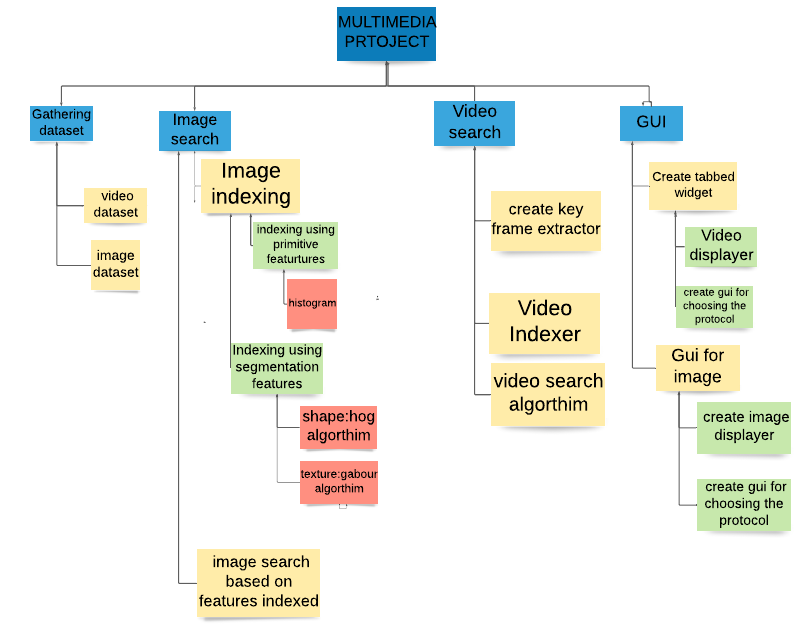
\includegraphics[width=120mm,height=60mm]{fig/25.png}
			\caption{DB EER Diagram }
			\label{DB EER Diagram }
		\end{figure}
	\begin{figure}[H]
		\centering
		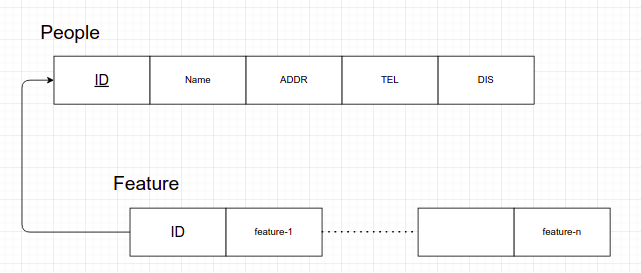
\includegraphics[width=120mm,height=60mm]{fig/24.png}
		\caption{Database Schema   }
		\label{Database Schema }
	\end{figure}
	\end{itemize}



\begin{figure}[H]
	\centering
	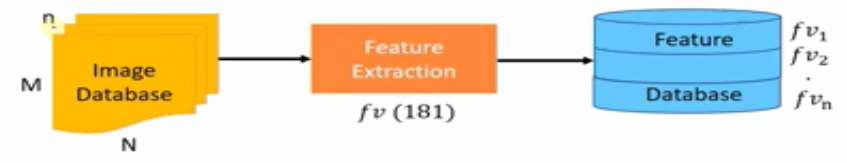
\includegraphics[width=120mm,height=60mm]{fig/21.png}
	\caption{image feature exract diagram }
	\label{image feature exract diagram}
\end{figure}
\begin{figure}[H]
	\centering
	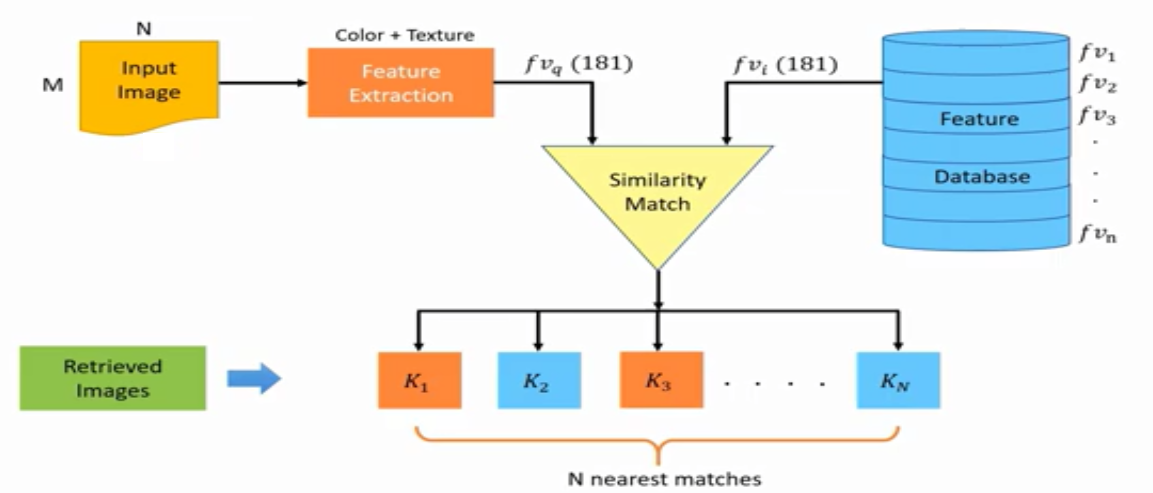
\includegraphics[width=120mm,height=60mm]{fig/20.png}
	\caption{image query diagram }
	\label{image query diagram}
\end{figure}
	\pagebreak
	\section{System design}
	\begin{enumerate}
		\item  \textbf{{\large system database}}\\
		in this project we have a database for images which has a CSV file each one store features for all techniques.
		
		
		\item \textbf{{\large user UI}} \\
		this is a GUI the user interact with to make queries.
		\item \textbf{{\large the processing part}}\\
		this part is responsible to process images according to the selected technique.
		\item \textbf{{\large  operating scenario}}\\
		 first we build our database for  images for all technique and then select from GUI  image search if image user select the technique and the image want to search with. all data from GUI is passed to the processing part to give results and print it in the GUI  
		
	\end{enumerate}
	
	
	 
	
	
	
	\pagebreak
	\section{Testing scenarios and results}
	\begin{itemize}
		\item search for one member of team  using his old pic and we get the younger pic that stored in our DB
	
	\begin{figure}[H]
		\centering
		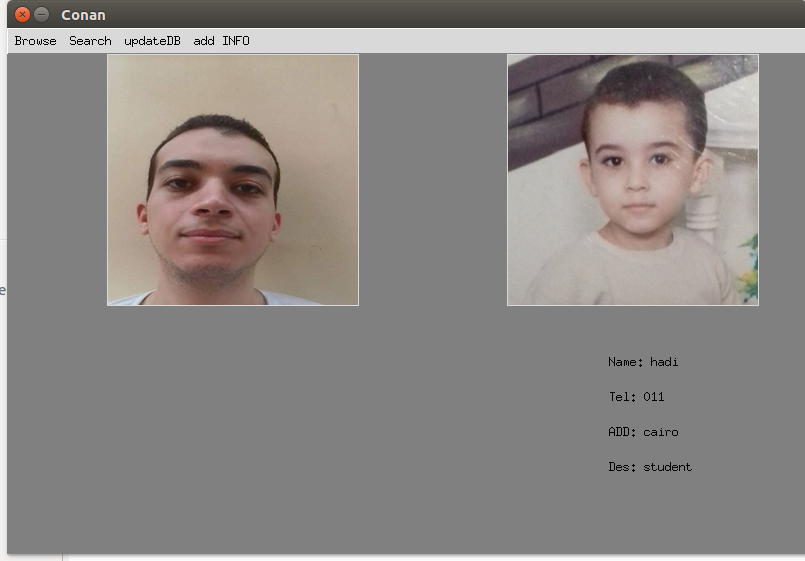
\includegraphics[width=120mm,height=60mm]{fig/17.png}
		%\caption{image feature exract diagram }
		%\label{image feature exract diagram}
	\end{figure}
	
		\item search for one member of team  using his old pic that has some animation as noise and we get the younger pic that stored in our DB 
	\begin{figure}[H]
	\centering
	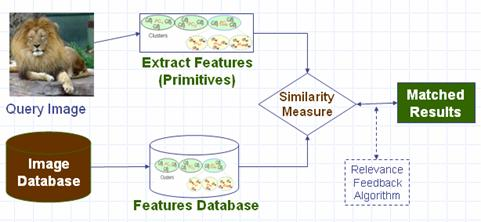
\includegraphics[width=120mm,height=60mm]{fig/18.png}
	%\caption{image feature exract diagram }
	%\label{image feature exract diagram}
\end{figure}
\pagebreak
	\item search for one member of team  using his old pic that scanned from mobile and we get the younger pic that stored in our DB
	\begin{figure}[H]
	\centering
	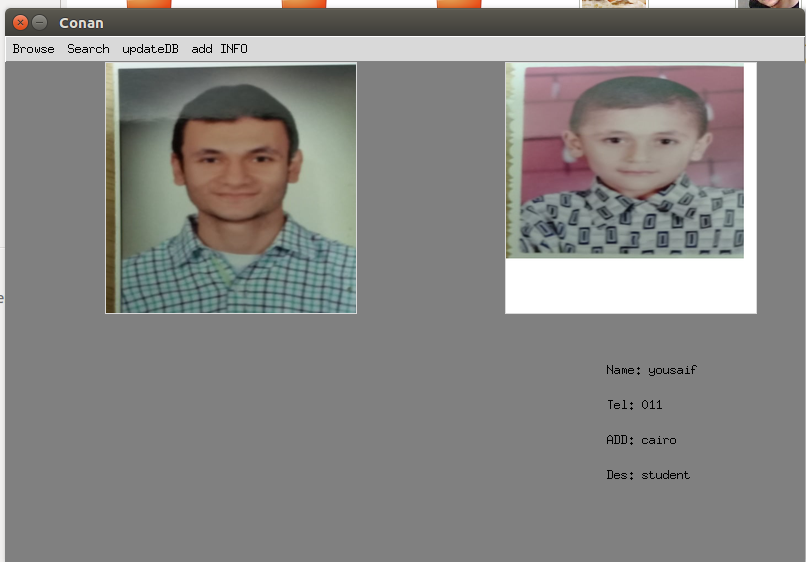
\includegraphics[width=120mm,height=60mm]{fig/14.png}
	%\caption{image feature exract diagram }
	%\label{image feature exract diagram}
\end{figure}
	\item search for one member of team  using his old pic that scanned using digital scanner and we get the younger pic that stored in our DB
			\begin{figure}[H]
			\centering
			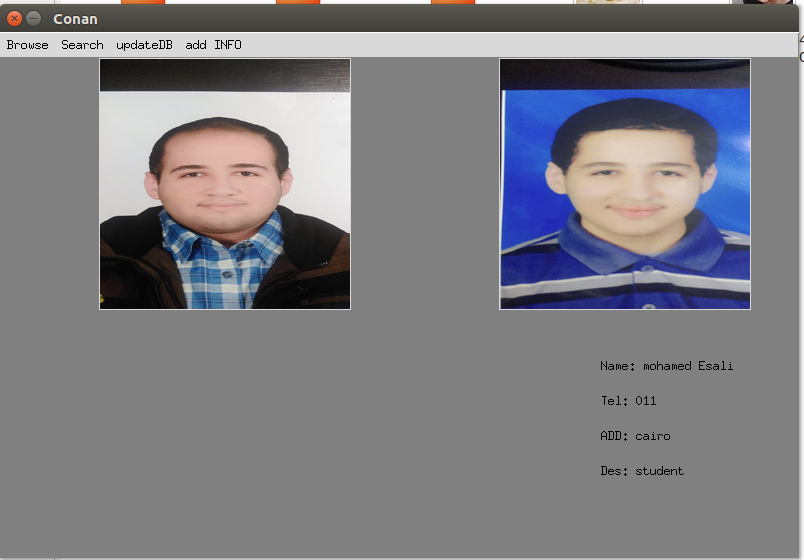
\includegraphics[width=120mm,height=60mm]{fig/15.png}
			%\caption{image feature exract diagram }
			%\label{image feature exract diagram}
		\end{figure}
	\pagebreak
		\item search for one member of team  using his old pic  that taking by digital camera and we get the younger pic that stored in our DB
	\begin{figure}[H]
	\centering
	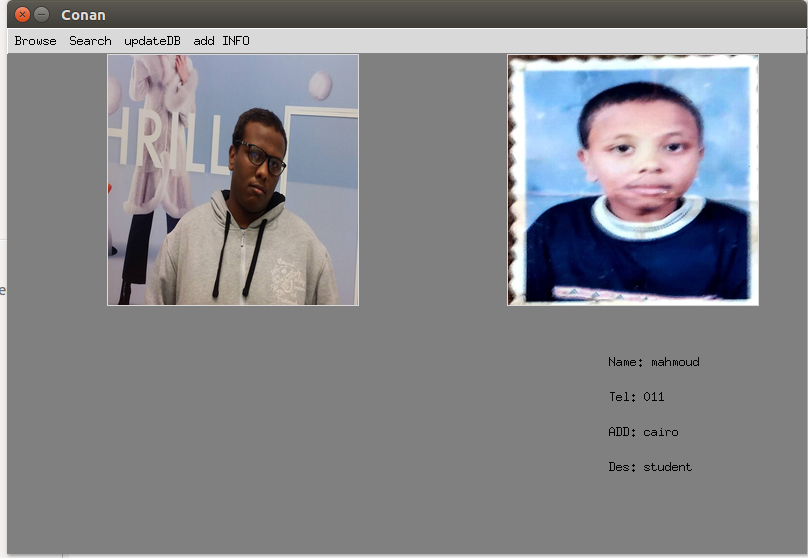
\includegraphics[width=120mm,height=60mm]{fig/16.png}
	%\caption{image feature exract diagram }
	%\label{image feature exract diagram}
\end{figure}
	\item search for an actress using her old pic and we get the younger pic that stored in our DB
	\begin{figure}[H]
	\centering
	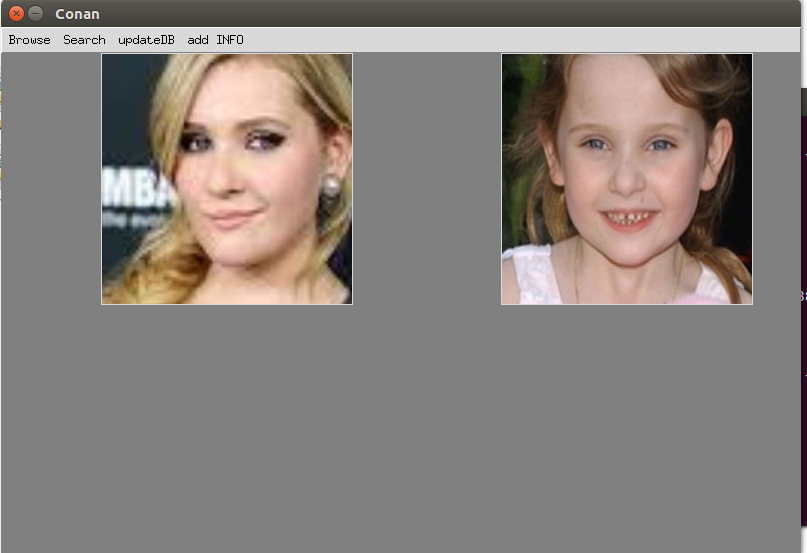
\includegraphics[width=120mm,height=60mm]{fig/10.png}
	%\caption{image feature exract diagram }
	%\label{image feature exract diagram}
\end{figure}
\pagebreak
	\item search for an actor  using his old pic and we get the younger pic that stored in our DB even if it is black and white
	\begin{figure}[H]
	\centering
	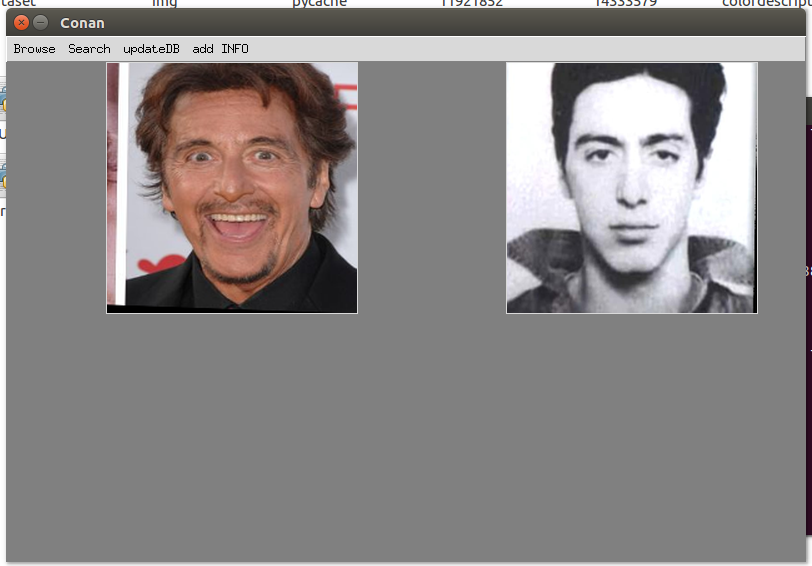
\includegraphics[width=120mm,height=60mm]{fig/11.png}
	%\caption{image feature exract diagram }
	%\label{image feature exract diagram}
\end{figure}
\item search for an actor  using his old pic and we get the younger pic that stored in our DB 
	\begin{figure}[H]
	\centering
	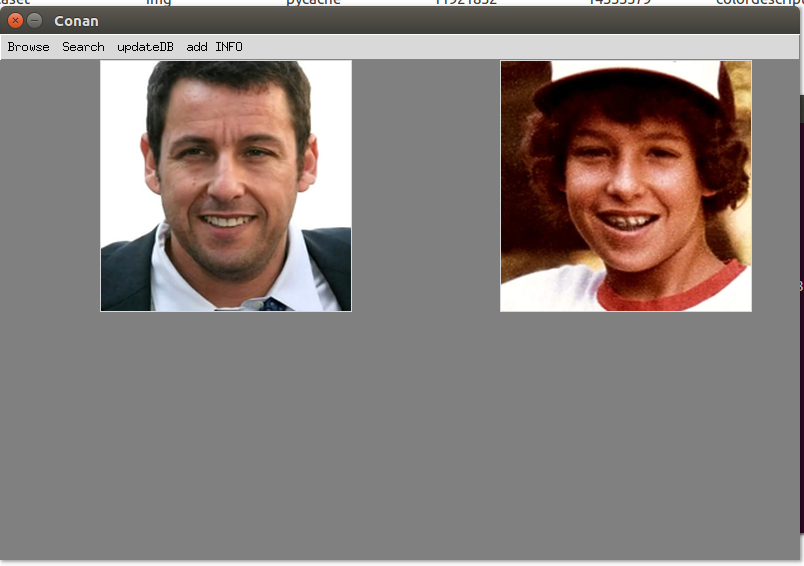
\includegraphics[width=120mm,height=60mm]{fig/12.png}
	%\caption{image feature exract diagram }
	%\label{image feature exract diagram}
\end{figure}
\pagebreak
\item search for an actress  using her old pic and we get the younger pic that stored in our DB 
	\begin{figure}[H]
	\centering
	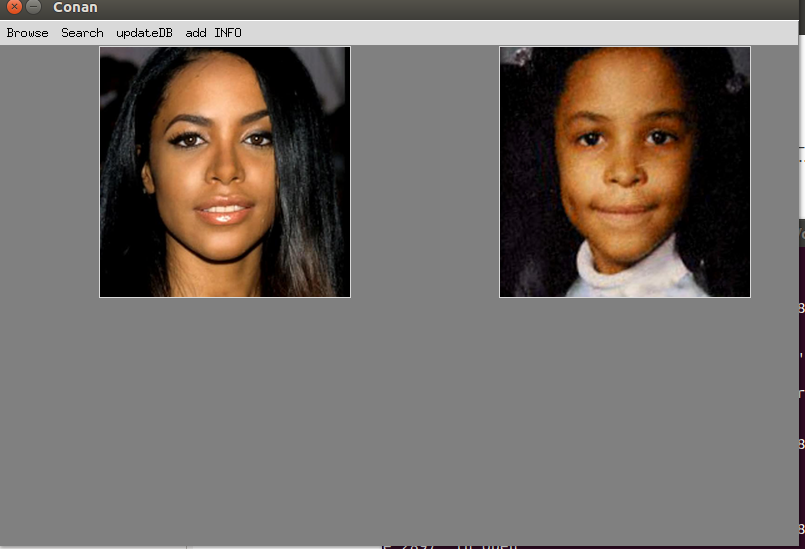
\includegraphics[width=120mm,height=60mm]{fig/13.png}
	%\caption{image feature exract diagram }
	%\label{image feature exract diagram}
\end{figure}
\end{itemize}
	\pagebreak
	\section{End user guide}
	\begin{enumerate}
		\item This is the primitive user interface.
			\begin{figure}[H]
			\centering
			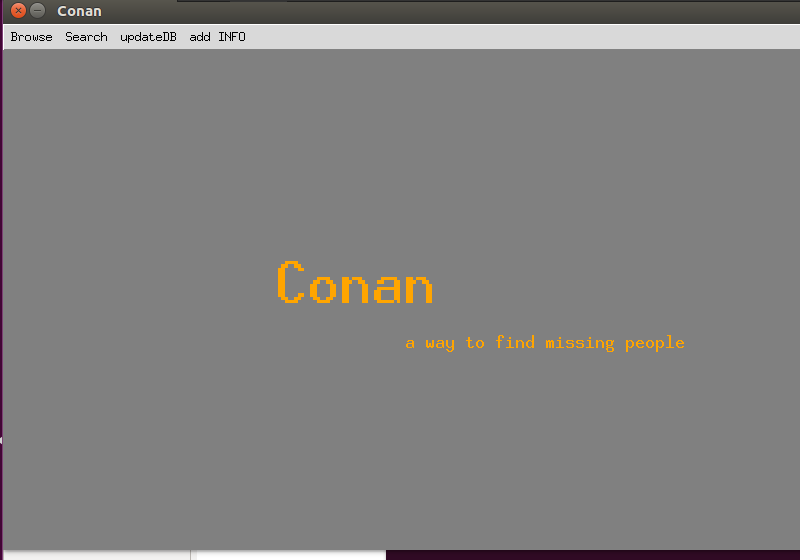
\includegraphics[width=120mm,height=60mm]{fig/00.png}
			%\caption{image feature exract diagram }
			%\label{image feature exract diagram}
		\end{figure}
		
	\pagebreak
	\item before to go in query we need to build database first so go from  updateDB
			
		\begin{figure}[H]
		\centering
		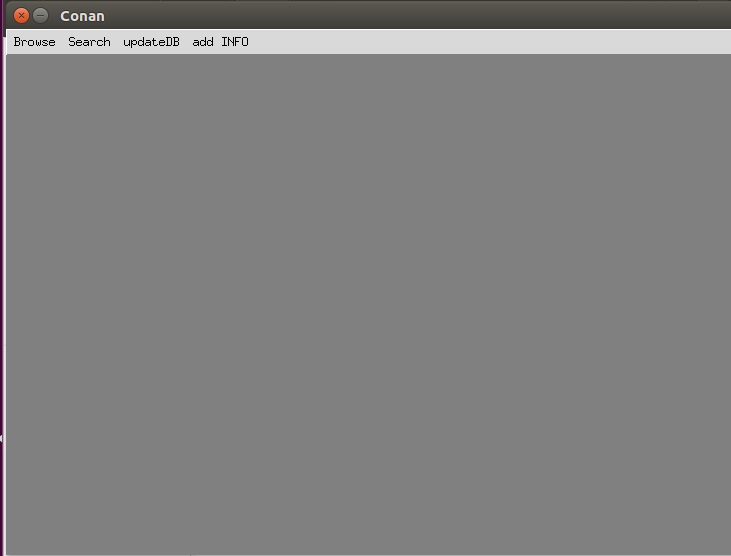
\includegraphics[width=120mm,height=60mm]{fig/01.png}
		%\caption{image feature exract diagram }
		%\label{image feature exract diagram}
	\end{figure}
		\item 	It may take a time and give you alert message for waiting.
	\begin{figure}[H]
	\centering
	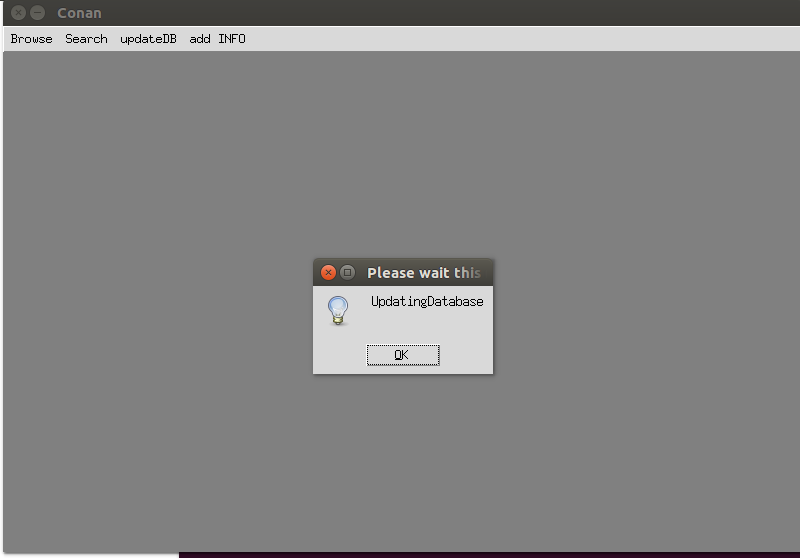
\includegraphics[width=120mm,height=60mm]{fig/2.png}
	%\caption{image feature exract diagram }
	%\label{image feature exract diagram}
\end{figure}
	
	
	\pagebreak
			\item 	When the database is finished updating, a message Database Status will appear.
		\begin{figure}[H]
		\centering
		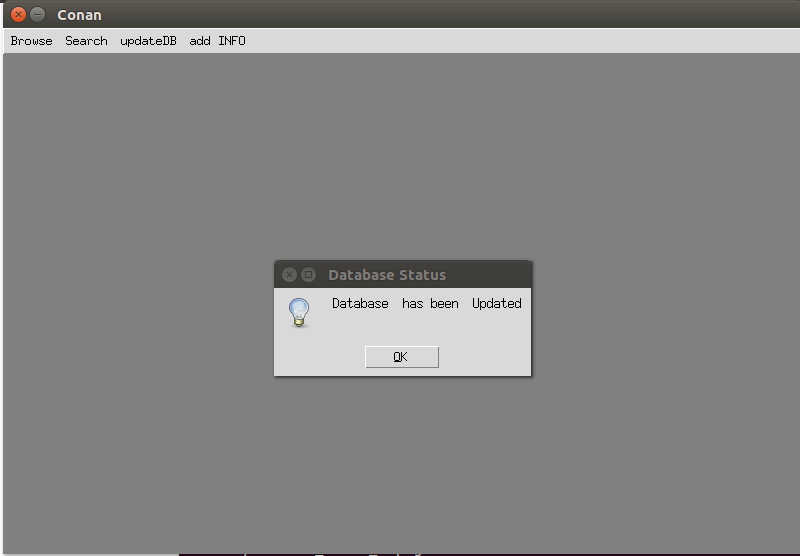
\includegraphics[width=120mm,height=60mm]{fig/3.png}
		%\caption{image feature exract diagram }
		%\label{image feature exract diagram}
	\end{figure}
	
	
	
	
	
	
	
	
		\item now we can search for any image we want From Browse choose Image ex Image. 
		
			\begin{figure}[H]
			\centering
			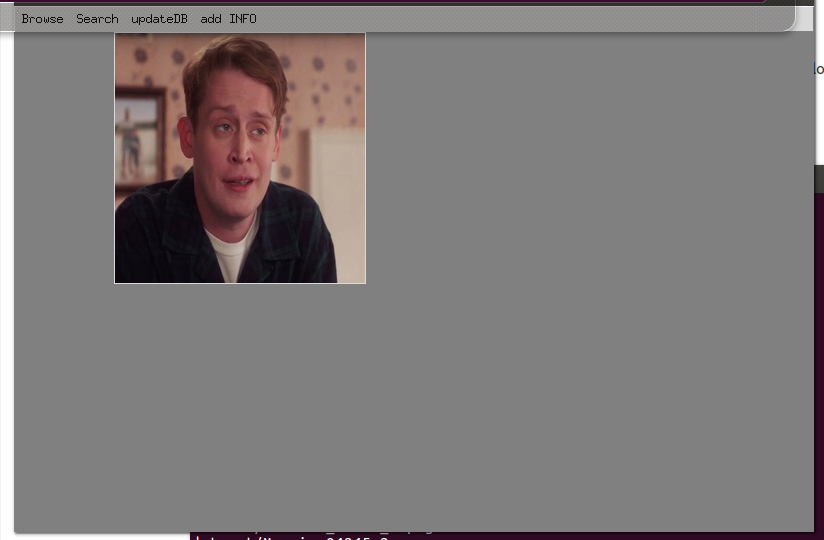
\includegraphics[width=120mm,height=60mm]{fig/4.png}
			%\caption{image feature exract diagram }
			%\label{image feature exract diagram}
		\end{figure}


\pagebreak
		\item 	to get the result Click on search button and the result will appear in the area for displaying results, and when you click at any result image it will be  standalone
		\begin{figure}[H]
		\centering
		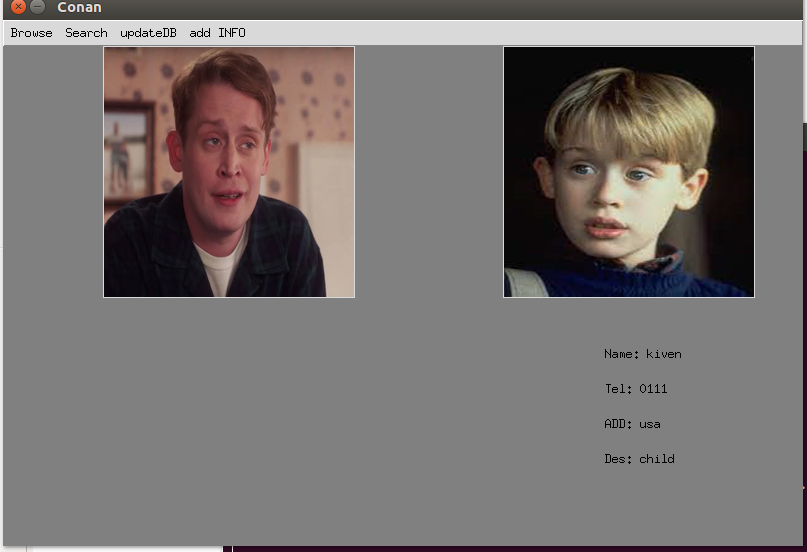
\includegraphics[width=120mm,height=60mm]{fig/05.png}
		%\caption{image feature exract diagram }
		%\label{image feature exract diagram}
	\end{figure}


	
	\item to enter information to image click to add INFO.
		
		 	\begin{figure}[H]
		 	\centering
		 	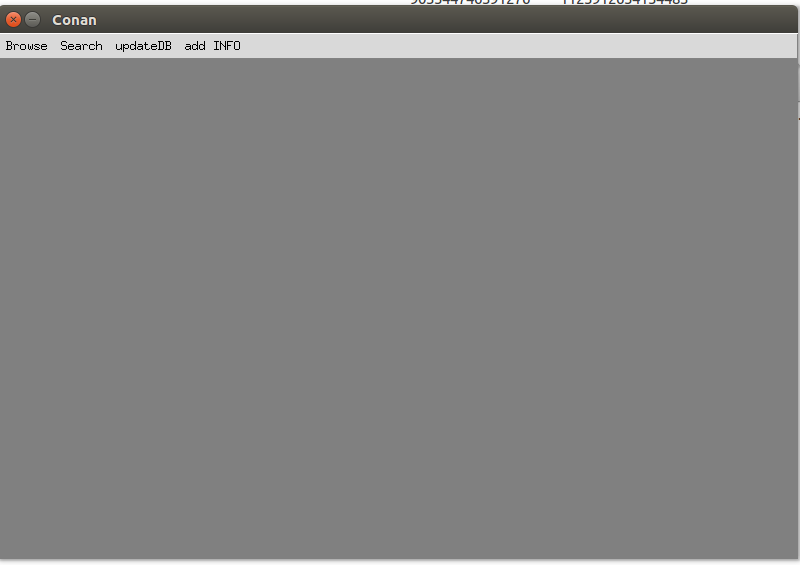
\includegraphics[width=120mm,height=60mm]{fig/06.png}
		 	%\caption{image feature exract diagram }
		 	%\label{image feature exract diagram}
		 \end{figure}
	
	
	\pagebreak
		\item 	another page will appear to enter information in diffrant fields.
			\begin{figure}[H]
			\centering
			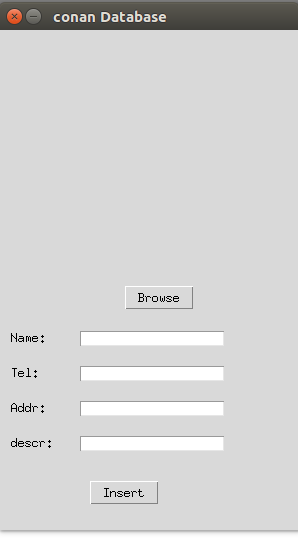
\includegraphics[width=60mm,height=60mm]{fig/7.png}
			%\caption{image feature exract diagram }
			%\label{image feature exract diagram}
		\end{figure}
	
		\begin{figure}[H]
		\centering
		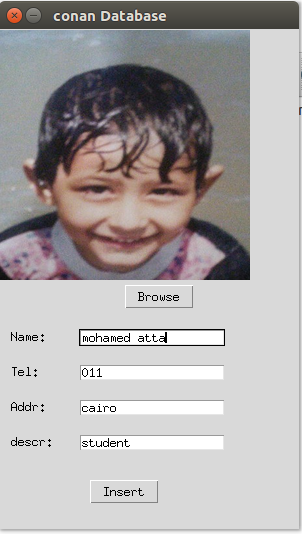
\includegraphics[width=60mm,height=60mm]{fig/09.png}
		%\caption{image feature exract diagram }
		%\label{image feature exract diagram}
	\end{figure}
		\begin{figure}[H]
		\centering
		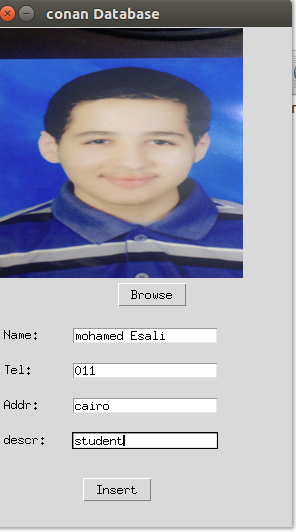
\includegraphics[width=60mm,height=60mm]{fig/08.png}
		%\caption{image feature exract diagram }
		%\label{image feature exract diagram}
	\end{figure}
		\begin{figure}[H]
		\centering
		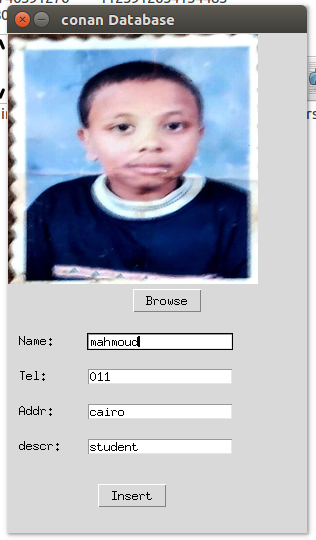
\includegraphics[width=50mm,height=60mm]{fig/07.png}
		%\caption{image feature exract diagram }
		%\label{image feature exract diagram}
	\end{figure}
	\begin{figure}[H]
	\centering
	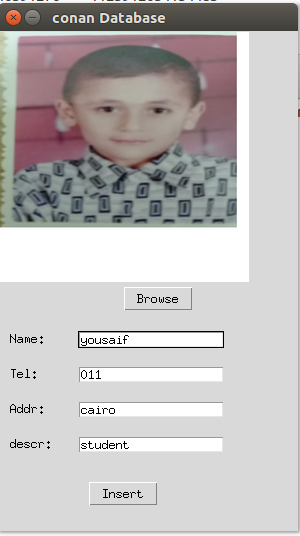
\includegraphics[width=60mm,height=50mm]{fig/6.png}
	%\caption{image feature exract diagram }
	%\label{image feature exract diagram}
\end{figure}
	\begin{figure}[H]
	\centering
	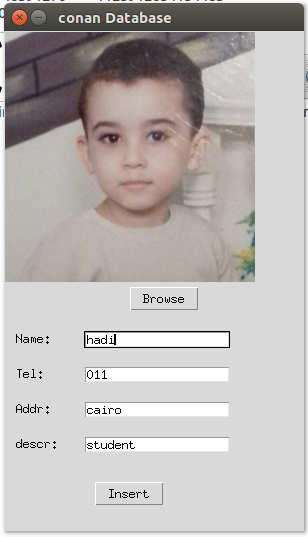
\includegraphics[width=60mm,height=50mm]{fig/04.png}
	%\caption{image feature exract diagram }
	%\label{image feature exract diagram}
\end{figure}
	\item 	When finshed  entering info , a message Status will appear.
		\begin{figure}[H]
		\centering
		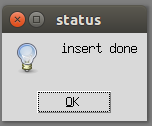
\includegraphics[width=60mm,height=20mm]{fig/8.png}
		%\caption{image feature exract diagram }
		%\label{image feature exract diagram}
	\end{figure}

						
	\end{enumerate}
\pagebreak

	\pagebreak
	\section{Conclusion}
	Finally, Conan application has been able to recongize missing people even if they have different ages.
	


	

	\pagebreak	
%	\addcontentsline{toc}{section}{References}
%	\bibliography{ref.bib} 
%	\bibliographystyle{ieeetr}
	
	
	\printglossary
\end{document}
